% Provenance (never printed): old seconde/premiere S material on the ocean
% (the ocean as a layered fluid, its heat, upwelling and productive waters);
% see sources/book2/PROVENANCE.md. All profiles are WOA23 columns, all
% densities the EOS-80 one-atmosphere equation, computed in
% figdata/grade-10/ocean_profiles.py.
\chapter{المحيط الطبقي}\label{ch:g10:layered-ocean}

في يوم صيفي تسبح مبتعدًا عن الشاطئ في ماء دافئ لطيف. ثم تدلّي ساقيك --- فتلاقي
قدماك ماء باردًا فجأة، على بعد مترين أو نحوهما تحت السطح. فالبحر ليس ممتزجًا من
أعلاه إلى أسفله: بل يتكون من طبقات، دافئة وخفيفة في الأعلى، وباردة وكثيفة في
الأسفل. وفي عرض المحيط يمتد هذا \omterm{def:g10:layered-ocean:stratification}{التطبق} نفسه إلى عمق كيلومترات، وهو الذي يقرر أين
يكون البحر صحراء وأين يعج بالحياة. يتناول هذا الفصل المحيط في عمقه: كيف يُقاس،
وكيف تتغير درجة حرارته وملوحته نحو الأسفل، ولماذا تكون الطبقات مستقرة، وأين يعود
الماء العميق البارد صاعدًا إلى السطح.

\begin{recall}
يحتوي ماء البحر على أملاح ذائبة: وملوحته، نحو 35 غرامًا من الملح لكل كيلوغرام من
ماء البحر في المتوسط، تختلف من بحر إلى آخر. وتحرك الرياح التيارات السطحية والدوامات
الدائرية الكبرى؛ وتتحرك تيارات عميقة من الماء البارد المالح ببطء على امتداد قاع
المحيط (الكتاب 1، الصف 8). والكثافة هي الكتلة مقسومة على الحجم (كتب الفيزياء).
والعوالق النباتية، وهي طحالب مجهرية، تحتاج إلى الضوء وإلى مغذيات معدنية لتنمو
بالتركيب الضوئي، وهي تغذي بقية السلاسل الغذائية في المحيط (كتب الأحياء).
\end{recall}

\section{قياس المحيط}

يغطي المحيط نحو \num{362}~مليون~\unit{km^2}، ومتوسط عمقه
\qty{3682}{m}: أي نحو \num{1.33}~مليار~\unit{km^3} من الماء. ومعظمه يقع بعيدًا تحت
مدى الضوء، ولا يمكن قياسه إلا بإنزال أجهزة إليه.
% ledger: charette:ocean-volume

من السفينة، يُنزل علماء المحيطات بكابل إطارًا يحمل مجسات تقيس ناقلية الماء (التي
تُحسب منها ملوحته)، ودرجة حرارته، والضغط (ومنه العمق)، وتحيط به حلقة من القوارير
تُغلق عند أعماق مختارة لإعادة عينات من الماء إلى السفينة. ومنذ عام 2000 أضاف أسطول
من العوامات الآلية ملايين المقاطع الرأسية: فكل عوامة تنجرف مع التيارات على عمق
\qty{1000}{m}، وتغوص كل عشرة أيام تقريبًا إلى \qty{2000}{m}، ثم تصعد إلى السطح
وهي تقيس درجة الحرارة والملوحة في طريقها، وترسل مقطعها عبر
الأقمار الصناعية.
% ledger: argo:fleet

\begin{dated}{2026}
تضم شبكة «أرغو» الدولية قرابة 4000 عوامة عاملة؛ وقد جُمع مقطعها الرأسي
الثلاثة ملايين في يوليو 2024.
% ledger: argo:fleet
\end{dated}

\begin{omfigure}
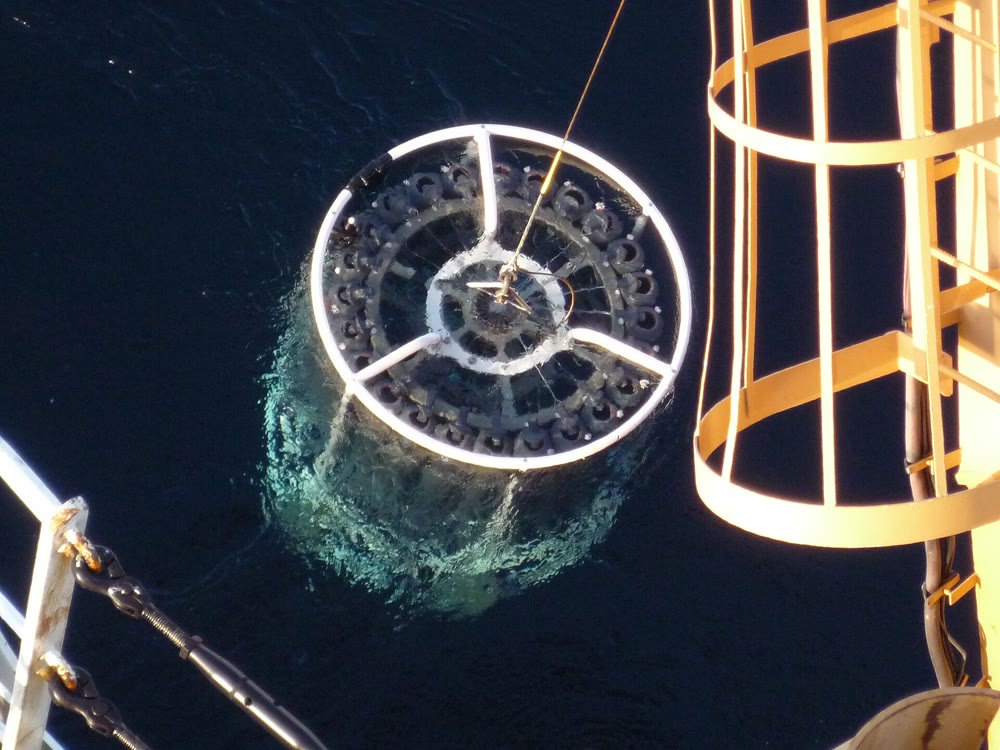
\includegraphics[height=4.4cm]{images/book2/g10-noaa-ctd-rosette.jpg}\hspace{0.4cm}%
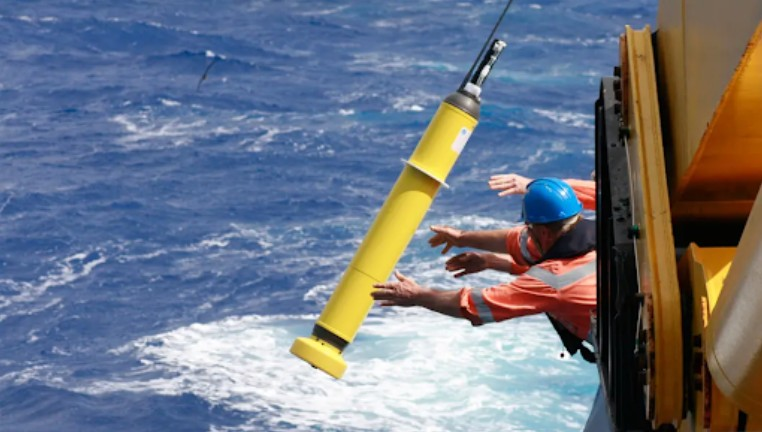
\includegraphics[height=4.4cm]{images/book2/g10-noaa-argo-float.jpg}

{\small في اليمين: حلقة من قوارير أخذ العينات حول مجساتها، تُرفع إلى جانب سفينة
أبحاث في المحيط المتجمد الشمالي، 2008 (الصورة: بابلو كليمنتي--كولون، مكتبة
صور الإدارة الوطنية للمحيطات والغلاف الجوي). في اليسار: إطلاق عوامة لقياس المقاطع
من سفينة أبحاث (الصورة: برنامج رصد المحيط العالمي ومراقبته التابع للإدارة الوطنية
للمحيطات والغلاف الجوي). كلتاهما ملك عام.}
\end{omfigure}

تعطي هذه المقاطع، متوسطةً على عقود من القياسات، صورة للمحيط في عمقه. ومقاطع هذا
الفصل من هذه المتوسطات، مأخوذة من \emph{أطلس المحيط العالمي 2023} الصادر عن
المراكز الوطنية للمعلومات البيئية التابعة للإدارة الوطنية للمحيطات والغلاف
الجوي.

\section{درجة الحرارة مع العمق}

\begin{omfigure}
\begin{tikzpicture}
\begin{axis}[omrecord, omdepth, width=0.62\linewidth, height=8.2cm,
  axis x line=top, xmin=-3, xmax=31, ymin=0, ymax=2000,
  xlabel={\foreignlanguage{arabic}{درجة الحرارة \babelsublr{(\unit{\degreeCelsius})}}}, ylabel={\foreignlanguage{arabic}{العمق \babelsublr{(\unit{m})}}},
  tick label style={font=\small}, label style={font=\small},
  legend style={font=\scriptsize, at={(0.98,0.03)}, anchor=south east}]
\addplot[omThm!85!black, thick] table[x=t, y=depth] {figdata/out/grade-10-ocean_profiles-site-warmpool.dat};
\addplot[omDef!85!black, thick] table[x=t, y=depth] {figdata/out/grade-10-ocean_profiles-site-atlantic.dat};
\addplot[black!70, thick, dashed] table[x=t, y=depth] {figdata/out/grade-10-ocean_profiles-site-arctic.dat};
\legend{{\foreignlanguage{arabic}{المحيط الهادئ المداري، \babelsublr{5.5\textdegree} ش}}, {\foreignlanguage{arabic}{شمال الأطلسي، \babelsublr{40.5\textdegree} ش}}, {\foreignlanguage{arabic}{المحيط المتجمد الشمالي، \babelsublr{75.5\textdegree} ش}}}
\node[font=\scriptsize, anchor=west] (ml) at (axis cs:21,430) {الطبقة المختلطة};
\draw[black!50] (ml.north east) -- (axis cs:28.9,35);
\node[font=\scriptsize, anchor=west] (tc) at (axis cs:15.5,600) {طبقة التدرج الحراري};
\draw[black!50] (tc.north) -- (axis cs:19.9,150);
\node[font=\scriptsize, anchor=west] at (axis cs:7,1500) {المحيط العميق};
\end{axis}
\end{tikzpicture}

{\small متوسط درجة الحرارة بحسب العمق في ثلاثة مواقع (يزداد العمق نحو الأسفل).
البيانات: أطلس المحيط العالمي 2023، متوسطات سنوية، المراكز الوطنية للمعلومات البيئية.}
\end{omfigure}
% ledger: data:b2-woa23 (profiles in figdata/grade-10/ocean_profiles.py)

يسخّن ضوء الشمس المحيط من الأعلى، في طبقته السطحية. وتقلّب الرياح والأمواج هذا
الماء الدافئ فتجعله طبقة شبه متجانسة الحرارة. وتحتها تنخفض درجة الحرارة سريعًا على
مدى بضع مئات من الأمتار؛ وأعمق من ذلك تنخفض ببطء حتى الماء البارد الذي يملأ أحواض
المحيط.

\begin{definition}[الطبقة المختلطة]\label{def:g10:layered-ocean:mixed-layer}
\emph{الطبقة المختلطة}\index{طبقة مختلطة} هي الطبقة السطحية من المحيط، التي تقلّبها
الرياح والأمواج، والتي لا تكاد درجة الحرارة والملوحة تتغيران فيها مع
العمق.
\end{definition}

\begin{definition}[طبقة التدرج الحراري؛ طبقة التدرج الملحي؛ طبقة التدرج الكثافي؛ المحيط العميق]\label{def:g10:layered-ocean:thermocline}
\emph{طبقة التدرج الحراري}\index{طبقة التدرج الحراري} هي الطبقة الواقعة تحت \omterm{def:g10:layered-ocean:mixed-layer}{الطبقة
المختلطة}، التي تنخفض فيها درجة الحرارة سريعًا مع العمق. والطبقة التي تتغير فيها
الملوحة سريعًا مع العمق هي \emph{طبقة تدرج ملحي}\index{طبقة التدرج الملحي}؛
والطبقة التي تزداد فيها الكثافة سريعًا مع العمق هي
\emph{طبقة التدرج الكثافي}\index{طبقة التدرج الكثافي}. وتحتها يقع \emph{المحيط
العميق}\index{محيط عميق}، البارد البطيء التغير.
\end{definition}

في المحيط الهادئ المداري تكون \omterm{def:g10:layered-ocean:mixed-layer}{الطبقة المختلطة} عند \qty{29.2}{\degreeCelsius}
وسماكتها نحو \qty{60}{m}؛ وبين \qty{70}{m} و\qty{300}{m} تنخفض درجة الحرارة
بقرابة تسع عشرة درجة، وعند \qty{1000}{m} لا تتجاوز
\qty{4.5}{\degreeCelsius}. وفي شمال الأطلسي يكون السطح أبرد والانخفاض أكثر تدرجًا.
وفي المحيط المتجمد الشمالي يبقى العمود كله في حدود درجتين من
\qty{0}{\degreeCelsius}: فلا طبقة سطحية دافئة تستحق
الذكر.
% ledger: data:b2-woa23

\begin{method}[قراءة مقطع رأسي للمحيط]\label{met:g10:layered-ocean:profile}
\begin{enumerate}
  \item حدد المحورين: يزداد العمق نحو الأسفل، وتُقرأ الكمية المقيسة على امتداد
        الأعلى.
  \item \omterm{def:g10:layered-ocean:mixed-layer}{الطبقة المختلطة} هي الجزء العلوي حيث يكون المنحنى شبه رأسي؛ وعمقها حيث يبدأ
        المنحنى بالانحناء (قاعدة شائعة: حيث تنخفض درجة الحرارة
        \qty{0.5}{\degreeCelsius} عن قيمتها عند السطح).
  \item \omterm{def:g10:layered-ocean:thermocline}{طبقة التدرج الحراري} هي حيث يكون المنحنى أقرب ما يكون إلى الأفقي: أكبر
        تغير في أصغر عمق.
  \item وفي الأسفل، اقرأ القيم العميقة وقارن المواقع عند العمق نفسه.
\end{enumerate}
\end{method}

تتغير \omterm{def:g10:layered-ocean:mixed-layer}{الطبقة المختلطة} مع الفصول. ففي الشتاء يفقد السطح حرارة، وتقلّب العواصف البحر،
فتتعمق \omterm{def:g10:layered-ocean:mixed-layer}{الطبقة المختلطة}؛ وفي الصيف تسخّن الشمس طبقة سطحية رقيقة لا تقدر الرياح
الألطف على مزجها نحو الأسفل، فتتكون \emph{طبقة تدرج حراري موسمية} قرب السطح ---
وهي الماء البارد الذي تلاقيه قدما السابح.

\begin{omfigure}
\begin{tikzpicture}
\begin{axis}[omrecord, omdepth, width=0.6\linewidth, height=6.6cm,
  axis x line=top, xmin=12, xmax=24, ymin=0, ymax=300,
  xlabel={\foreignlanguage{arabic}{درجة الحرارة \babelsublr{(\unit{\degreeCelsius})}}}, ylabel={\foreignlanguage{arabic}{العمق \babelsublr{(\unit{m})}}},
  tick label style={font=\small}, label style={font=\small},
  legend style={font=\scriptsize, at={(0.98,0.03)}, anchor=south east}]
\addplot[omDef!85!black, thick] table[x=t_feb, y=depth] {figdata/out/grade-10-ocean_profiles-season.dat};
\addplot[omThm!85!black, thick] table[x=t_aug, y=depth] {figdata/out/grade-10-ocean_profiles-season.dat};
\legend{فبراير, أغسطس}
\end{axis}
\end{tikzpicture}

{\small الشتاء والصيف في شمال الأطلسي (\qty{40.5}{\degree} ش،
\qty{30.5}{\degree} غ): متوسط درجات الحرارة الشهرية لفبراير وأغسطس.
في فبراير تبلغ \omterm{def:g10:layered-ocean:mixed-layer}{الطبقة المختلطة} نحو \qty{170}{m}؛ وفي أغسطس تستقر طبقة دافئة
سماكتها نحو \qty{15}{m} على طبقة تدرج حراري موسمية. البيانات: أطلس المحيط العالمي
2023، المراكز الوطنية للمعلومات البيئية.}
\end{omfigure}
% ledger: data:b2-woa23 (mixed-layer depths by the 0.5 degC rule, computed in figdata/grade-10/ocean_profiles.py)

\section{الملوحة والكثافة}

تتوقف كثافة ماء البحر على درجة حرارته وعلى ملوحته. وهي تُحسب بصيغة متفق عليها
دوليًا، هي معادلة حالة ماء البحر، المطابَقة على قياسات
مخبرية.

\begin{proposition}[كثافة ماء البحر]\label{prop:g10:layered-ocean:density}
تزداد كثافة ماء البحر بازدياد ملوحته وتنقص بارتفاع درجة حرارته. فعند ضغط السطح،
تبلغ كثافة ماء بحر ملوحته 35 \qty{1028.1}{kg/m^3} عند
\qty{0}{\degreeCelsius} و\qty{1023.3}{kg/m^3} عند \qty{25}{\degreeCelsius}؛ وتبلغ
كثافة الماء النقي عند \qty{4}{\degreeCelsius}
\qty{1000.0}{kg/m^3}.
\end{proposition}
% ledger: unesco:eos80 (values computed in figdata/grade-10/ocean_profiles.py)

\begin{omfigure}
\begin{tikzpicture}
\begin{axis}[omrecord, width=0.7\linewidth, height=6.2cm, xmin=-2, xmax=30,
  ymin=1016, ymax=1033, xlabel={\foreignlanguage{arabic}{درجة الحرارة \babelsublr{(\unit{\degreeCelsius})}}},
  ylabel={\foreignlanguage{arabic}{الكثافة \babelsublr{(\unit{kg/m^3})}}}, tick label style={font=\small},
  label style={font=\small}, yticklabel style={/pgf/number format/1000 sep={}}]
\addplot[omThm!85!black, thick] table[x=t, y=rho_s38] {figdata/out/grade-10-ocean_profiles-eos.dat};
\addplot[black!80, thick] table[x=t, y=rho_s35] {figdata/out/grade-10-ocean_profiles-eos.dat};
\addplot[omDef!85!black, thick] table[x=t, y=rho_s30] {figdata/out/grade-10-ocean_profiles-eos.dat};
\node[font=\scriptsize, anchor=south west, omThm!85!black] at (axis cs:1,1030.75) {\foreignlanguage{arabic}{الملوحة \babelsublr{38}}};
\node[font=\scriptsize, anchor=south west] at (axis cs:1,1028.35) {\foreignlanguage{arabic}{الملوحة \babelsublr{35}}};
\node[font=\scriptsize, anchor=south west, omDef!85!black] at (axis cs:1,1024.35) {\foreignlanguage{arabic}{الملوحة \babelsublr{30}}};
\end{axis}
\end{tikzpicture}

{\small كثافة ماء البحر عند ضغط السطح، بحسب درجة حرارته، لثلاث ملوحات (محسوبة
من المعادلة الدولية لحالة ماء البحر).}
\end{omfigure}
% ledger: unesco:eos80

يظهر أمران في المخطط. فكل وحدة ملوحة تضيف نحو
\qty{0.8}{kg/m^3}. وكل درجة احترار تنقص نحو \qty{0.31}{kg/m^3}
عند \qty{25}{\degreeCelsius}، و\qty{0.18}{kg/m^3} عند \qty{10}{\degreeCelsius}،
لكنها لا تنقص إلا \qty{0.06}{kg/m^3} قرب \qty{0}{\degreeCelsius}: ففي البحار
الدافئة تتحكم درجة الحرارة في الكثافة، وفي البحار الباردة تتحكم فيها الملوحة.
% ledger: unesco:eos80 (slopes computed in figdata/grade-10/ocean_profiles.py)

\begin{remark}
كثافات هذا الفصل محسوبة عند ضغط السطح. فضغط الماء الذي فوقه يضغط ماء البحر قليلًا،
بنحو \qty{4}{kg/m^3} لكل كيلومتر من العمق؛ ويقارن علماء المحيطات الكتل المائية
عند الضغط نفسه، كي لا تُحتسب إلا درجة الحرارة والملوحة.
\end{remark}
% ledger: unesco:eos80-checks (computed in figdata/grade-10/ocean_profiles.py: 3.9 kg/m3 per km from the 10000-dbar check values)

\begin{omfigure}
\begin{tikzpicture}
\begin{axis}[name=sal, omrecord, omdepth, width=0.5\linewidth, height=7.2cm,
  axis x line=top, xmin=27.5, xmax=37, ymin=0, ymax=1000,
  xlabel={الملوحة}, ylabel={\foreignlanguage{arabic}{العمق \babelsublr{(\unit{m})}}},
  tick label style={font=\small}, label style={font=\small}]
\addplot[omThm!85!black, thick] table[x=s, y=depth] {figdata/out/grade-10-ocean_profiles-site-warmpool.dat};
\addplot[omDef!85!black, thick] table[x=s, y=depth] {figdata/out/grade-10-ocean_profiles-site-atlantic.dat};
\addplot[black!70, thick, dashed] table[x=s, y=depth] {figdata/out/grade-10-ocean_profiles-site-arctic.dat};
\node[font=\scriptsize, anchor=west, align=left] at (axis cs:28.2,120) {طبقة التدرج\\الملحي القطبية};
\end{axis}
\begin{axis}[at={(sal.east)}, anchor=west, xshift=0.9cm, omrecord, omdepth,
  width=0.5\linewidth, height=7.2cm, axis x line=top, xmin=1021, xmax=1028.5, yticklabels={},
  ymin=0, ymax=1000, xlabel={\foreignlanguage{arabic}{الكثافة \babelsublr{(\unit{kg/m^3})}}},
  tick label style={font=\small}, label style={font=\small},
  xticklabel style={/pgf/number format/1000 sep={}},
  legend style={font=\scriptsize, at={(0.03,0.03)}, anchor=south west}]
\addplot[omThm!85!black, thick] table[x=rho, y=depth] {figdata/out/grade-10-ocean_profiles-site-warmpool.dat};
\addplot[omDef!85!black, thick] table[x=rho, y=depth] {figdata/out/grade-10-ocean_profiles-site-atlantic.dat};
\addplot[black!70, thick, dashed] table[x=rho, y=depth] {figdata/out/grade-10-ocean_profiles-site-arctic.dat};
\legend{المحيط الهادئ المداري, شمال الأطلسي, المحيط المتجمد الشمالي}
\end{axis}
\end{tikzpicture}

{\small الملوحة (في اليسار) والكثافة عند ضغط السطح (في اليمين) بحسب العمق، في
المواقع الثلاثة لمقاطع درجة الحرارة. وفي كل موقع تزداد الكثافة نحو الأسفل.
البيانات: أطلس المحيط العالمي 2023، المراكز الوطنية للمعلومات البيئية؛ والكثافات
من المعادلة الدولية لحالة ماء البحر.}
\end{omfigure}
% ledger: data:b2-woa23, unesco:eos80

في المحيط الهادئ المداري تنطبق \omterm{def:g10:layered-ocean:thermocline}{طبقة التدرج الكثافي} على \omterm{def:g10:layered-ocean:thermocline}{طبقة التدرج الحراري}. وفي
المحيط المتجمد الشمالي لا تكاد درجة الحرارة تتغير، لكن الملوحة ترتفع من 28 عند
السطح، حيث تخففها الأنهار والجليد الذائب، إلى 34.8 عند
\qty{500}{m}: \omterm{def:g10:layered-ocean:thermocline}{فطبقة التدرج الملحي} هي \omterm{def:g10:layered-ocean:thermocline}{طبقة التدرج الكثافي}. وفي كل حالة تزداد
الكثافة نحو الأسفل.
% ledger: data:b2-woa23

\begin{definition}[التطبق]\label{def:g10:layered-ocean:stratification}
يكون المحيط \emph{متطبقًا}\index{تطبق} حين تزداد كثافته مع العمق: فالماء الأخف
يستقر فوق الماء الأكثف، في طبقات.
\end{definition}

المحيط المتطبق مستقر. فكتلة الماء المدفوعة نحو الأسفل إلى ماء أكثف تكون أخف من
محيطها فتطفو عائدة؛ والكتلة المدفوعة نحو الأعلى تغوص عائدة. ولمزج الطبقات، يجب على
الريح أن تعمل ضد ذلك، وكلما كانت \omterm{def:g10:layered-ocean:thermocline}{طبقة التدرج الكثافي} أقوى، صار ذلك أصعب: \omterm{def:g10:layered-ocean:thermocline}{فطبقة
التدرج الحراري} غطاء يفصل السطح عن \omterm{def:g10:layered-ocean:thermocline}{المحيط العميق}. ويمتلئ \omterm{def:g10:layered-ocean:thermocline}{المحيط العميق} بماء غاص منذ
زمن بعيد من البحار القطبية الباردة، حيث يصير الماء السطحي كثيفًا بما يكفي ليغوص
(الكتاب 1، الصف 8).

\section{الانبثاق}

\begin{definition}[الانبثاق]\label{def:g10:layered-ocean:upwelling}
\emph{الانبثاق}\index{انبثاق} هو صعود ماء بارد من تحت الطبقة السطحية، ليحل محل
ماء سطحي تدفعه الريح بعيدًا. ويحدث على امتداد بعض السواحل وفي عرض
المحيط.
\end{definition}
% ledger: noaa:upwelling

على امتداد ساحل ما، تجر الريح الهابة موازية للشاطئ الماء السطحي؛ وبسبب دوران
الأرض لا يتبع الماء الريح ببساطة بل ينحرف عنها، نحو اليمين في نصف الكرة الشمالي
ونحو اليسار في نصف الكرة الجنوبي (وكيفية ذلك موضوع المجلدات الجامعية). وقبالة
بيرو تهب الريح على امتداد الشاطئ نحو خط الاستواء، فيُدفع الماء السطحي نحو عرض
البحر؛ ويصعد ماء بارد قرب الساحل ليحل محله. ويحدث \omterm{def:g10:layered-ocean:upwelling}{الانبثاق} أيضًا على امتداد خط
الاستواء، حيث تدفع الرياح التجارية الماء السطحي بعيدًا عنه من الجانبين.
% ledger: noaa:upwelling, kessler:peru-upwelling

\begin{omfigure}
\begin{tikzpicture}[font=\footnotesize, >={Stealth[length=2mm]}]
  % ocean and thermocline
  \fill[omDef!12] (0,-3.2) rectangle (8.2,0);
  \fill[omDef!30] (0,-3.2) -- (0,-2.0) .. controls (3,-2.0) and (5.5,-1.6) .. (7.4,-0.35) -- (8.2,0) -- (8.2,-3.2) -- cycle;
  \draw[omDef!80!black, dashed] (0,-2.0) .. controls (3,-2.0) and (5.5,-1.6) .. (7.4,-0.35);
  \node[anchor=north west, omDef!80!black] at (0.1,-2.05) {طبقة التدرج الحراري};
  \node[anchor=west, black!70] at (0.15,-0.9) {ماء سطحي دافئ};
  \node[anchor=west, black!70] at (0.15,-2.75) {ماء بارد غني بالمغذيات};
  % land
  \fill[omExo!30, draw=black!60] (7.0,-3.2) -- (8.2,-0.1) -- (8.6,0.0) -- (9.6,1.2) -- (10.6,2.2) -- (10.6,-3.2) -- cycle;
  \node[anchor=south, align=center] at (9.9,-1.6) {اليابسة};
  % surface flow and rising water
  \draw[->, thick, omThm!80!black] (7.2,-0.3) -- (3.6,-0.3);
  \node[anchor=south, omThm!80!black] at (5.4,-0.25) {ماء سطحي يُدفع نحو عرض البحر};
  \foreach \x/\y in {6.1/-2.1, 6.8/-1.7} \draw[->, thick, omDef!80!black] (\x,\y) -- (\x+0.45,\y+1.15);
  \node[anchor=north, omDef!80!black, align=center] at (6.0,-2.25) {ماء بارد يصعد};
  % wind along the shore, northward: with west on the left and east on the
  % right the reader looks north, so the wind goes into the page
  \draw[black!70, thick] (2.6,1.0) circle (0.22);
  \draw[black!70, thick] (2.6,1.0) ++(45:0.22) -- ++(225:0.44) (2.6,1.0) ++(135:0.22) -- ++(315:0.44);
  \node[anchor=west, align=left] at (2.9,1.0) {ريح موازية للشاطئ نحو خط الاستواء\\أي نحو الشمال، داخلةً في الصفحة};
  \node[anchor=north west, black!60] at (0,-3.25) {الغرب $\leftarrow$};
  \node[anchor=north east, black!60] at (10.6,-3.25) {$\rightarrow$ الشرق};
\end{tikzpicture}

{\small \omterm{def:g10:layered-ocean:upwelling}{الانبثاق} الساحلي قبالة بيرو (مقطع عرضي تخطيطي من الغرب إلى الشرق، بغير
مقياس): تهب الريح على امتداد الشاطئ نحو خط الاستواء، نحو الشمال، داخلةً في الصفحة؛
فينحرف الماء السطحي إلى يسارها ويُدفع نحو عرض البحر؛ ويصعد ماء بارد من تحت \omterm{def:g10:layered-ocean:thermocline}{طبقة
التدرج الحراري} قرب الساحل ليحل محله.}
\end{omfigure}

الماء الذي يصعد ليس باردًا فحسب. فتحت الطبقة السطحية المضاءة بالشمس، تحرر بقايا
العوالق الميتة التي تغوص وتتحلل المغذيات المعدنية التي تحتاج إليها العوالق
النباتية. وحين تعود هذه المغذيات إلى الضوء، تجعل مناطق \omterm{def:g10:layered-ocean:upwelling}{الانبثاق} أخصب مياه المحيط،
وفيها أغنى مصايد الأسماك. وحيث يكون المحيط شديد \omterm{def:g10:layered-ocean:stratification}{التطبق} ولا شيء يرفع الماء العميق،
تنفد المغذيات من الطبقة المضاءة: فمراكز الدوامات شبه المدارية هي صحارى
المحيط.
% ledger: noaa:upwelling

\begin{omfigure}
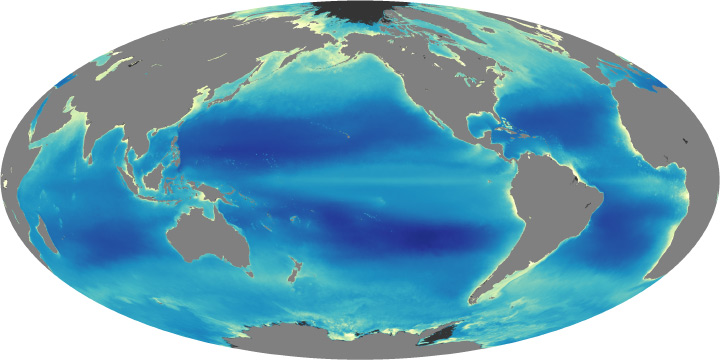
\includegraphics[width=0.8\linewidth]{images/book2/g10-nasa-ocean-chlorophyll.jpg}

{\small يخضور العوالق النباتية كما يُرى من الفضاء، متوسطًا على 2002--2010: من
الأزرق الداكن (قليل جدًا) عبر الأزرق الفاتح إلى الأصفر (كثير)؛ واليابسة بالرمادي.
ويبرز ساحل بيرو والشريط الممتد على خط الاستواء في المحيط الهادئ؛ والدوامات زرقاء
داكنة. الصورة: جيسي ألين وروبرت سيمون، مرصد الأرض التابع لناسا
(ملك عام).}
\end{omfigure}

\begin{omfigure}
\begin{tikzpicture}
\begin{axis}[omrecord, omdepth, width=0.6\linewidth, height=7.2cm,
  axis x line=top, xmin=4, xmax=26, ymin=0, ymax=600,
  xlabel={\foreignlanguage{arabic}{درجة الحرارة \babelsublr{(\unit{\degreeCelsius})}}}, ylabel={\foreignlanguage{arabic}{العمق \babelsublr{(\unit{m})}}},
  tick label style={font=\small}, label style={font=\small},
  legend style={font=\scriptsize, at={(0.98,0.03)}, anchor=south east}]
\addplot[omExo!85!black, thick] table[x=t, y=depth] {figdata/out/grade-10-ocean_profiles-site-peru.dat};
\addplot[omThm!85!black, thick] table[x=t, y=depth] {figdata/out/grade-10-ocean_profiles-site-gyre.dat};
\addplot[black!40, dashed, domain=0:600, samples=2] ({15}, {x});
\legend{{\foreignlanguage{arabic}{قبالة بيرو، \babelsublr{13.5\textdegree} ج}}, {\foreignlanguage{arabic}{دوامة جنوب المحيط الهادئ، \babelsublr{20.5\textdegree} ج}}}
\end{axis}
\end{tikzpicture}

{\small قبالة بيرو يقترب الماء البارد من السطح: فالماء عند
\qty{15}{\degreeCelsius} (الخط المتقطع) يقع على عمق نحو \qty{65}{m}، مقابل قرابة
\qty{300}{m} في وسط دوامة جنوب المحيط الهادئ، الأبعد عن خط الاستواء. البيانات:
أطلس المحيط العالمي 2023، متوسطات سنوية، المراكز الوطنية للمعلومات
البيئية.}
\end{omfigure}
% ledger: data:b2-woa23

\section{تمارين}

\begin{exercise}[$\star$]\label{exo:g10:layered-ocean:1}
عرّف \omterm{def:g10:layered-ocean:mixed-layer}{الطبقة المختلطة} \omterm{def:g10:layered-ocean:thermocline}{وطبقة التدرج الحراري}. وما الذي يقلّب \omterm{def:g10:layered-ocean:mixed-layer}{الطبقة المختلطة}؟
\end{exercise}

\begin{exercise}[$\star$]\label{exo:g10:layered-ocean:2}
عرّف \omterm{def:g10:layered-ocean:upwelling}{الانبثاق}. ولماذا تكون مياه مناطق \omterm{def:g10:layered-ocean:upwelling}{الانبثاق} غنية بالحياة؟
\end{exercise}

\begin{exercise}[$\star$]\label{exo:g10:layered-ocean:3}
باستعمال مقاطع درجة الحرارة في المواقع الثلاثة، أعطِ درجة الحرارة عند السطح وعند
\qty{1000}{m} في المحيط الهادئ المداري وفي المحيط المتجمد
الشمالي.
\end{exercise}

\begin{exercise}[$\star$]\label{exo:g10:layered-ocean:4}
أيهما أكثف: ماء بحر ملوحته 35 عند \qty{25}{\degreeCelsius} أم عند
\qty{0}{\degreeCelsius}؟ وماء بحر ملوحته 35 أم الماء النقي، عند درجة الحرارة
نفسها؟ استعمل قيم الفصل.
\end{exercise}

\begin{exercise}[$\star$]\label{exo:g10:layered-ocean:5}
فسّر كيف تقيس عوامة المقاطع مقطعًا رأسيًا للمحيط، ولماذا تفيد العوامات حيث نادرًا
ما تذهب السفن.
\end{exercise}

\begin{exercise}[$\star\star$]\label{exo:g10:layered-ocean:6}
يغطي المحيط \num{361.84}~مليون~\unit{km^2} بعمق متوسط قدره
\qty{3682}{m}. احسب حجمه بالكيلومترات المكعبة. وما الكسر من عمقه الذي يمثله
أعلى \qty{100}{m}؟
\end{exercise}

\begin{exercise}[$\star\star$]\label{exo:g10:layered-ocean:7}
في مقطع شمال الأطلسي لشهر أغسطس، تبلغ درجة الحرارة
\qty{22.7}{\degreeCelsius} عند السطح، و\qty{22.2}{\degreeCelsius} عند
\qty{15}{m}، و\qty{21.8}{\degreeCelsius} عند \qty{20}{m}،
و\qty{17.3}{\degreeCelsius} عند \qty{50}{m}. باستعمال قاعدة الطريقة، قدّر عمق
\omterm{def:g10:layered-ocean:mixed-layer}{الطبقة المختلطة}. وما متوسط معدل انخفاض درجة الحرارة بين \qty{20}{m} و\qty{50}{m}،
بالدرجات لكل متر؟
\end{exercise}

\begin{exercise}[$\star\star$]\label{exo:g10:layered-ocean:8}
في موقع شمال الأطلسي نفسه يكون السطح عند \qty{15.3}{\degreeCelsius}
في فبراير و\qty{22.7}{\degreeCelsius} في أغسطس، بينما يكون عند \qty{300}{m}
في \qty{13.5}{\degreeCelsius} في الشهرين كليهما. فسّر لماذا لا يتبع الماء العميق
الفصول، ولماذا تكون \omterm{def:g10:layered-ocean:mixed-layer}{الطبقة المختلطة} في الشتاء أعمق بكثير منها في
الصيف.
\end{exercise}

\begin{exercise}[$\star\star$]\label{exo:g10:layered-ocean:9}
قرب \qty{10}{\degreeCelsius}، تضيف وحدة ملوحة واحدة
\qty{0.78}{kg/m^3} إلى الكثافة وتنقص درجة احترار واحدة
\qty{0.18}{kg/m^3}. كم درجة احترار تلغي وحدة ملوحة واحدة؟ أجب عن السؤال نفسه قرب
\qty{0}{\degreeCelsius}، حيث لا تنقص الدرجة الواحدة إلا \qty{0.06}{kg/m^3}. وماذا
تستنتج بالنسبة إلى البحار
القطبية؟
\end{exercise}

\begin{exercise}[$\star\star$]\label{exo:g10:layered-ocean:10}
في المحيط المتجمد الشمالي يكون الماء عند السطح في \qty{-1.4}{\degreeCelsius}
وملوحته 28.1، وعند \qty{200}{m} في \qty{-1.4}{\degreeCelsius}
وملوحته 33.3. وكثافتاهما \qty{1022.6}{kg/m^3}
و\qty{1026.8}{kg/m^3}. ما الذي يجعل الماء الأعمق أكثف؟ وسمِّ الطبقة
الواقعة بينهما.
\end{exercise}

\begin{exercise}[$\star\star$]\label{exo:g10:layered-ocean:11}
فسّر لماذا يكون المحيط المتطبق مستقرًا، مستعينًا بكتلة من الماء السطحي تدفعها موجة
نحو الأسفل.
\end{exercise}

\begin{exercise}[$\star\star\star$]\label{exo:g10:layered-ocean:12}
لتر من ماء بحر ملوحته 35 عند \qty{0}{\degreeCelsius} يُسخَّن إلى
\qty{25}{\degreeCelsius}. باستعمال كثافات الفصل، احسب كتلته، ثم حجمه الجديد. وبكم
تمدد، بالمليلترات؟ وطبقة من المحيط سماكتها \qty{700}{m} تسخن بالنسبة نفسها: فبكم
تزداد سماكتها؟ (وهذه مبالغة كبيرة في احترار المحيط الفعلي، لا تُستعمل هنا إلا
لإظهار الأثر.)
\end{exercise}

\begin{exercise}[$\star\star\star$]\label{exo:g10:layered-ocean:13}
في المحيط الهادئ المداري تبلغ الكثافة \qty{1021.6}{kg/m^3} عند \qty{50}{m}
و\qty{1026.0}{kg/m^3} عند \qty{200}{m}؛ وفي شمال الأطلسي في فبراير لا تكاد
درجة الحرارة تتغير على مدى أعلى \qty{150}{m}. ففي أيهما يسهل على عاصفة
أن تقلّب الماء حتى عمق \qty{150}{m}؟ فسّر.
\end{exercise}

\begin{exercise}[$\star\star\star$]\label{exo:g10:layered-ocean:14}
على خريطة اليخضور، حدد منطقتين عاليتي اليخضور في عرض المحيط بعيدًا عن أي ساحل،
ومنطقة واسعة شديدة الانخفاض في اليخضور. وباستعمال الفصل، فسّر كلًا
منها.
\end{exercise}

\begin{exercise}[$\star\star\star$]\label{exo:g10:layered-ocean:15}
افترض أن عوامة تغوص من \qty{1000}{m} إلى \qty{2000}{m} في ست
ساعات، ثم تصعد إلى السطح في عشر ساعات. احسب متوسط سرعتها الرأسية
في كل مرحلة، بالسنتيمترات في الثانية. وإذا قاست كل \qty{2}{s} في أثناء
صعودها، فكم قياسًا يحتوي المقطع، وما
العمق الذي يفصل بين قياسين منها في المتوسط؟
\end{exercise}

\section{مسألة: إنزال للمجسات قبالة بيرو}

\begin{problem}[{مسألة نهاية الأسبوع --- مقطعان رأسيان من جنوب المحيط الهادئ}]
\label{pb:g10:layered-ocean:1}
% ledger: data:b2-woa23, unesco:eos80 (values rounded from figdata/grade-10/ocean_profiles.py)
يعطي الجدول متوسط درجة الحرارة والملوحة، والكثافة المحسوبة عند ضغط السطح، في
مكانين من جنوب المحيط الهادئ: قبالة بيرو (\qty{13.5}{\degree} ج، \qty{77.5}{\degree} غ)
وفي وسط الدوامة شبه المدارية (\qty{20.5}{\degree} ج، \qty{110.5}{\degree} غ).

\begin{center}
\small
\begin{tabular}{c|ccc|ccc}
\hline
 & \multicolumn{3}{c|}{قبالة بيرو} & \multicolumn{3}{c}{الدوامة} \\
العمق (\unit{m}) & \unit{\degreeCelsius} & الملوحة & \unit{kg/m^3} & \unit{\degreeCelsius} & الملوحة & \unit{kg/m^3} \\
\hline
0 & 19.0 & 35.08 & 1025.08 & 24.0 & 36.41 & 1024.71 \\
25 & 17.4 & 35.06 & 1025.47 & 23.9 & 36.39 & 1024.73 \\
50 & 15.8 & 35.03 & 1025.83 & 23.6 & 36.38 & 1024.80 \\
100 & 13.7 & 34.93 & 1026.20 & 22.6 & 36.27 & 1025.02 \\
200 & 12.4 & 34.89 & 1026.44 & 20.3 & 35.80 & 1025.30 \\
300 & 11.1 & 34.80 & 1026.62 & 14.4 & 34.76 & 1025.92 \\
500 & 7.9 & 34.60 & 1026.97 & 7.1 & 34.39 & 1026.92 \\
\hline
\end{tabular}
\end{center}

\medskip
\noindent\textbf{الجزء الأول --- قراءة المقاطع.}
\begin{enumerate}
  \item أي الموقعين أدفأ عند السطح، وبكم؟
  \item أي الموقعين أبعد عن خط الاستواء؟ وهل فرق درجة حرارة السطح هو ما تتوقعه من
        خطي العرض وحدهما؟
  \item باستعمال قاعدة الطريقة، قدّر عمق \omterm{def:g10:layered-ocean:mixed-layer}{الطبقة المختلطة}
        في الدوامة.
  \item هل توجد \omterm{def:g10:layered-ocean:mixed-layer}{طبقة مختلطة} قبالة بيرو؟ صِف أعلى \qty{100}{m}.
  \item بين أي عمقين تنخفض درجة الحرارة أسرع ما يكون في الدوامة؟
        أعطِ المعدل، بالدرجات لكل مئة متر.
  \item على أي عمق تقريبًا يقع الماء الذي حرارته \qty{15}{\degreeCelsius} في
        كل موقع؟
\end{enumerate}

\medskip
\noindent\textbf{الجزء الثاني --- الكثافات.}
\begin{enumerate}[resume]
  \item تحقق من أن الكثافة تزداد مع العمق في الموقعين. وماذا يخبرك ذلك عن
        استقرارهما؟
  \item في الدوامة، الماء السطحي أشد ملوحة منه قبالة بيرو. فهل ينبغي أن يجعله ذلك
        أكثف أم أخف؟ وهل هو أكثف؟
  \item فسّر أي الأثرين يغلب.
  \item احسب ازدياد الكثافة من السطح إلى \qty{200}{m}
        قبالة بيرو.
  \item احسب الازدياد نفسه في الدوامة.
\end{enumerate}

\medskip
\noindent\textbf{الجزء الثالث --- مقارنة التطبق.}
\begin{enumerate}[resume]
  \item في الدوامة، أين يقع معظم ازدياد الكثافة في أعلى
        \qty{500}{m}: فوق \qty{200}{m} أم تحتها؟
  \item وقبالة بيرو، أين يقع؟
  \item عند \qty{500}{m}، قارن الموقعين. وماذا يوحي ذلك عن
        الماء العميق تحتهما كليهما؟
  \item فسّر في بضع جمل كيف رُفعت \omterm{def:g10:layered-ocean:thermocline}{طبقة التدرج الحراري} قبالة بيرو نحو
        السطح.
  \item تعيش العوالق النباتية في بضع عشرات الأمتار العليا. ففي أي موقع يكون
        الماء الغني بالمغذيات القادم من تحت \omterm{def:g10:layered-ocean:thermocline}{طبقة التدرج الحراري} في متناول
        تقليب الريح؟ فسّر.
\end{enumerate}

\medskip
\noindent\textbf{الجزء الرابع --- لماذا مياه بيرو خصبة.}
\begin{enumerate}[resume]
  \item كيف سيكون الماء السطحي قبالة بيرو لو توقفت الريح الموازية للشاطئ عن الهبوب
        شهورًا؟
  \item باستعمال خريطة اليخضور، قارن الموقعين.
  \item فسّر لماذا تُسمّى الدوامة صحراء المحيط مع أنها غارقة في ضوء
        الشمس.
  \item احسب نسبة ازديادَي الكثافة من السطح إلى
        \qty{200}{m} قبالة بيرو وفي الدوامة، وقل ماذا تُظهر.
\end{enumerate}
\end{problem}
